\section{Análise Exploratória}

A Análise Exploratória de Dados (AED) é uma etapa do fluxo de aprendizado de máquina que permite realizar uma exploração dos dados baseada em técnicas da Estatística Descritiva. Para essa etapa da pesquisa foi utilizado o notebook \textbf{analise-exploratoria.ipynb}. Por se tratar de uma atividade interativa, a utilização de um Jupyter Notebook se mostrou mais eficiente do que a utilização direta de um script Python.

\subsection{Valores Ausentes}

A primeira investigação realizada foi a busca de valores valores ausentes. Foram encontrados 1.900 segmentos com valores ausentes para o atributo txt\textunderscore seg. Nos demais atributos não havia valores ausentes. A tabela \ref{tab:valores-ausentes} apresenta a quantidade de segmentos com valores ausentes por tipo de segmento.

\begin{table}[h] 
\caption{Valores ausentes por tipo de segmento}
\label{tab:valores-ausentes}
	\begin{center} 
		\begin{tabular}{|l|r|} 
			\hline TIPO DE SEGMENTO & VALORES AUSENTES \\
			\hline
			\hline Anexo & 1.778 \\
			\hline Não Identificado & 95 \\			
			\hline Fecho & 21 \\
			\hline Ementa & 2 \\			
			\hline Artigo & 2 \\
			\hline Título & 1 \\
			\hline Alínea & 1 \\			
			\hline
		\end{tabular}
	\end{center}
	\fdp
\end{table} 

Os segmentos do tipo Anexo representam 93,57\% dos segmentos com valores ausentes. Como esse tipo de segmento representa arquivos binários associados aos atos, todos os segmentos desse tipo podem ser descartados. Além dos 1.778 apresentados na tabela \ref{tab:valores-ausentes}, existem outros 5.771 segmentos do tipo anexo com texto desprezível (ponto, vírgula, nome de arquivo, etc) totalizando 7.549 segmentos selecionados para exclusão durante a etapa de limpeza de dados. Os demais segmentos com valores ausentes representam 0.06\% do total (122/198.939) e foram também selecionados para exclusão.

Além dos valores ausentes, em diversos tipos de segmento foram identificados caracteres inválidos que precisaram ser removidos no processo de limpeza de dados, especialmente os caracteres de \textit{escape} e \textit{tags} HTML (exemplos: <br/>, \&ccedil, \&atilde).

\subsection{Distribuições de Atos e Segmentos}

Um aspecto que chamou a atenção na exploração dos dados foi a predominância de Atos Declaratórios Executivos (ADE), representando 71,79\% (14.948 dos 20.821 atos analisados), seguido pelas Soluções de Consulta (SC) com 14,98\% e Portarias (PORT) com 10,60\%. Os demais tipos de ato representam juntos 2.63\% do total. A figura \ref{fig:atos-por-tipo-ato} evidencia essa distribuição.

\begin{figure}[h]
	\caption{Quantidade de atos por tipo de ato}
	\center
	\label{fig:atos-por-tipo-ato}
	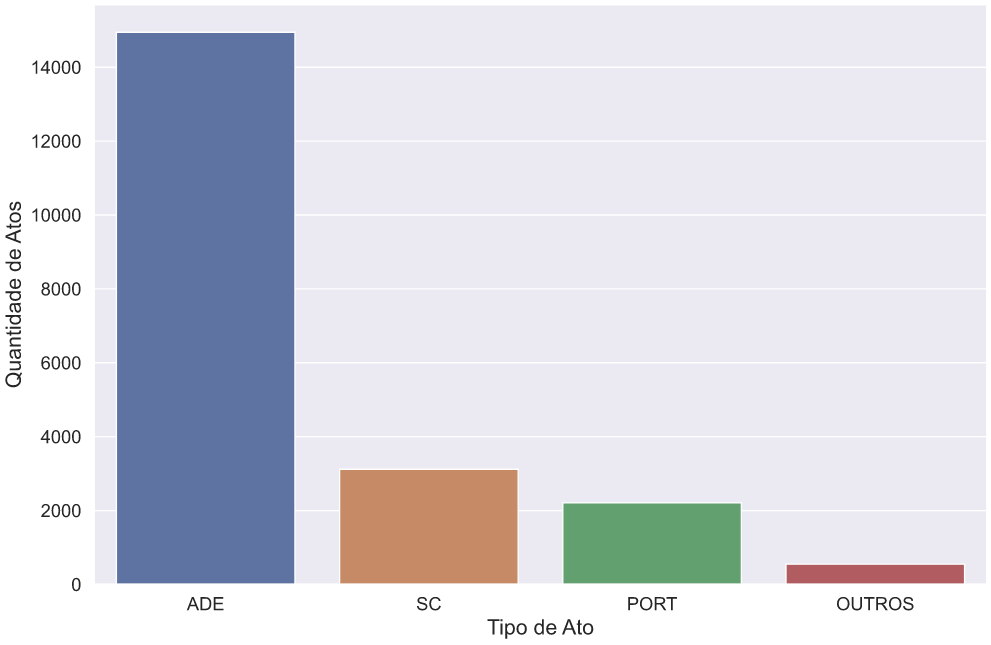
\includegraphics[scale=1.9]{exploratoria/atos-por-tipo-ato.png}
	\fdp
\end{figure}

Outro aspecto importante analisado foi a distribuição dos segmentos por tipo de ato e tipo de segmento. Na tabela \ref{tab:segmentos-por-tipo} é possível perceber que dos 17 tipos possíveis de segmento, somente 13 estão presentes em atos dos tipos ADE, SC e PORT. Além disso, nem todos os 13 tipos de segmento estão presentes nos 3 tipos de ato e alguns tipos de segmento são pouco frequentes.

\begin{table}[h] 
\caption{Quantidade de segmentos por tipo de ato e tipo de segmento}
\label{tab:segmentos-por-tipo}
	\begin{center} 

		\begin{tabular}{rrrr}
		\toprule
		TIPO DE ATO &      ADE    &   PORT &      SC \\
		TIPO DE SEGMENTO          &        &         \\
		\midrule
		Alínea           &    780 &  2.265 &      87 \\
		Artigo           & 37.921 & 11.578 &       3 \\
		Autor            &      3 &      4 &       0 \\
		Capítulo         &      5 &    381 &       0 \\
		Ementa           & 14.948 &  2.207 &   3.119 \\
		Fecho            & 14.853 &  2.289 &     919 \\
		Inciso           &  4.134 & 17.399 &       0 \\
		Item             &    398 &    388 &      10 \\
		Não Identificado & 36.288 & 11.726 &   6.609 \\
		Parágrafo        &    861 &  5.894 &       0 \\
		Seção            &      3 &    219 &       0 \\
		SubSeção         &      0 &     18 &       0 \\
		Título           &    545 &    540 &       0 \\
		\bottomrule
	\end{tabular}
	\end{center}
	\fdp
\end{table} 

Os segmentos do tipo ``Não Identificado'' representam um ponto de atenção para a classificação dos segmentos. Por ser o tipo padrão de segmento do sistema Normas, sempre que ocorre falha humana por omissão na classificação manual, o segmento fica classificado como ``Não Identificado''. Apesar disso, essa é uma classe válida de segmento amplamente utilizada para representar trechos do ato que não precisam de formatação específica. Por estar entre os tipos mais frequentes de segmento e ser um tipo válido, os segmentos desse tipo não podem ser removidos do escopo da classificação, mas a presença de segmentos com classificação omissa pode prejudicar os resultados dos modelos.

\subsection{Identificação de Padrões}

Ao longo da análise exploratória foram identificados, em alguns tipos de segmento, padrões de texto  que podem ser utilizados como heurísticas baseadas em expressões regulares. Se essas heurísticas apresentarem resultados melhores do que o modelo de classificação, será possível retirar alguns tipos de segmento do escopo da classificação, deixando o modelo mais específico para as demais classes. A seguir são apresentados os padrões encontrados:

\begin{alineas}
	\item Ementas podem ser iniciadas por um verbo ou pela expressão ``Assunto: ''. Exemplo: ``Cancela o registro especial para estabelecimento que realiza operação com papel[...]'';
	\item Artigos iniciam com a abreviação ``Art.'' seguida de um numeral ordinal. Exemplo: ``Art. 2\textsuperscript{o} O detalhamento do motivo da exclusão poderá ser obtido[...]'';
	\item Incisos são iniciados com um numeral romano seguido de hífem. Exemplo: ``IV – Fundamento legal para reconhecimento do direito[...]'';
	\item Alíneas iniciam com letras (minúsculas ou maiúsculas) seguidas de parênteses. Exemplo: ``f) desempenhar as tarefas inerentes ao sistema de progressão funcional[...]'';
	\item Parágrafos podem ser iniciados com a expressão ``Parágrafo único'' ou com o símbolo ``§'' seguido de um numeral ordinal. Exemplo: ``§ 2\textsuperscript{o} Compete à chefia imediata a gestão da frequência dos seus servidores[...]'';
	\item Fechos são iniciados com nomes próprios, seguidos ou não pelo cargo.
\end{alineas}

    
